\section{Introduction}

The work introduced in this chapter is the first main contribution of this dissertation. It is inspired by Radford et al. \cite{radford_2017}, which fine-tuned an LSTM LM with an extra linear layer to classify sentiment in text. This fine-tuning procedure highlighted that most of the sentiment signal was stored in a single neuron. Thus, this neuron could be directly adjusted to control the original LSTM LM to generate text with a target sentiment. This chapter shows an application of Radford et al. \cite{radford_2017}'s method to control sentiment in symbolic music generated via LMs. First, the VGMIDI dataset is introduced, a new dataset of symbolic piano pieces labeled according to a circumplex model of emotion. Second, an LSTM is trained as a LM with unlabeled piano pieces. Third, this LSTM-based LM is fine-tuned with an extra linear layer on the valence (i.e. sentiment) dimension of the VGMIDI dataset. Different than the findings of Radford et al. \cite{radford_2017}, the fine-tuning step didn't store the sentimental in a single neuron but in many neurons in a more balanced way. Thus, a genetic algorithm is applied to optimize the weights of these sentiment neurons towards a given sentiment. The accuracy of the model in classifying sentiment of symbolic music is evaluated with the VGMIDI dataset, and results show that the model is able to obtain good prediction accuracy. Moreover, a user study shows that human subjects agreed that the generated music has the intended sentiment; however, negative pieces can be ambiguous. This work has been published at the 20th annual conference of the International Society for Music Information Retrieval (ISMIR).

\section{The VGMIDI dataset}

% In order to apply the Radford et al. \cite{radford_2017} method to compose music with sentiment, we also need a dataset of MIDI files to train the LSTM and another one to train the logistic regression.
Currently, there are only a few datasets of symbolic music labelled according to emotion \cite{madhok2018sentimozart, tan2020automated, zhao2019emotional} and none are labelled according to sentiment. Thus, a new dataset called VGMIDI has been created with 823 pieces extracted from video game soundtracks in MIDI format. Video game soundtracks are well suited for this dataset because they are typically composed to intentionally keep the player in a specific affective state and thus tend to be less subjective. All the pieces are piano arrangements of the soundtracks and they vary in length from 26 seconds to 3 minutes. Among these pieces, 95 are annotated according to a circumplex model that represents emotion using a valence-arousal pair. VGMIDI uses a valence-arousal model because it allows continuous annotation of music and because of its flexibility---one can directly map a valence-arousal (v-a) pair to a multiclass (happy, sad, surprise, etc) or a binary (positive/negative) model. Thus, the same set of labelled data permits the investigation of affective algorithmic music composition as both a classification (multiclass and/or binary) and as a regression problem. The valence-arousal model is also one of the most common dimensional models used to label emotion in music \cite{Soleymani_2013}.

Annotating a piece according to the circumplex model consists of continuously listening to the piece and deciding what valence-arousal pair best represents the emotion of that piece in each moment, producing a time series of v-a pairs. This task is subjective, and hence there is no single ``correct'' time series for a given piece. Thus, VGMIDI  was labeled by asking several human subjects to listen to the pieces and then considering the average time series as the ground truth. This process was conducted online via Amazon Mechanical Turk, where each piece was annotated by 30 subjects using a web-based tool designed specifically for this task. Each subject annotated 2 pieces out of 95, and got rewarded USD \$0.50 for performing this task.

\subsection{Annotation Tool and Data Collection}
\label{sec:data_collection}

The tool designed to annotate the video game soundtracks in MIDI format is composed of five steps, each one being a single web page. These steps are based on the methodology proposed by Soleymani et al. \cite{Soleymani_2013} for annotating music pieces in audio waveform. First, participants are introduced to the annotation task with a short description explaining the goal of the task and how long it should take on average. Second, they are presented with the definitions of valence and arousal. On the same page, they are asked to play two short pieces and indicate whether arousal and valence are increasing or decreasing. Moreover, annotators are asked to write two to three sentences describing these short pieces. This page is intended to measure their understanding of the valence-arousal model and willingness to perform the task. Third, a video tutorial was made available to the annotators explaining how to use the annotation tool. Fourth, annotators are exposed to the main annotation page.

The main page has two phases: calibration and annotation. In the calibration phase, annotators listen to the first 15 seconds of the piece to get used to it and define the starting point of the annotation circle. In the annotation phase, they listen to the piece from beginning to end and label it using the annotation circle, which starts at the point defined during the calibration phase. Figure \ref{fig:annotation_main} shows the annotation interface for valence and arousal, where annotators click and hold the circle (with the play icon) inside the circumplex model (outer circle), indicating the current emotion of the piece. In order to maximize annotators' engagement in the task, the piece is only played while they maintain a click on the play circle. In addition, basic instructions on how to use the tool are shown to the participants along with the definitions of valence and arousal. A progression bar is also shown to the annotators to know how far they are from completing each phase. This last step (calibration and annotation) is repeated for a second piece. All of the pieces the annotators listened to are MIDI files synthesized with the ``Yamaha C5 Grand" soundfont. Finally, participants provide demographic information, including gender, age, location (country), musicianship experience, and whether they previously knew the pieces they annotated.

\begin{figure}
 \centering
 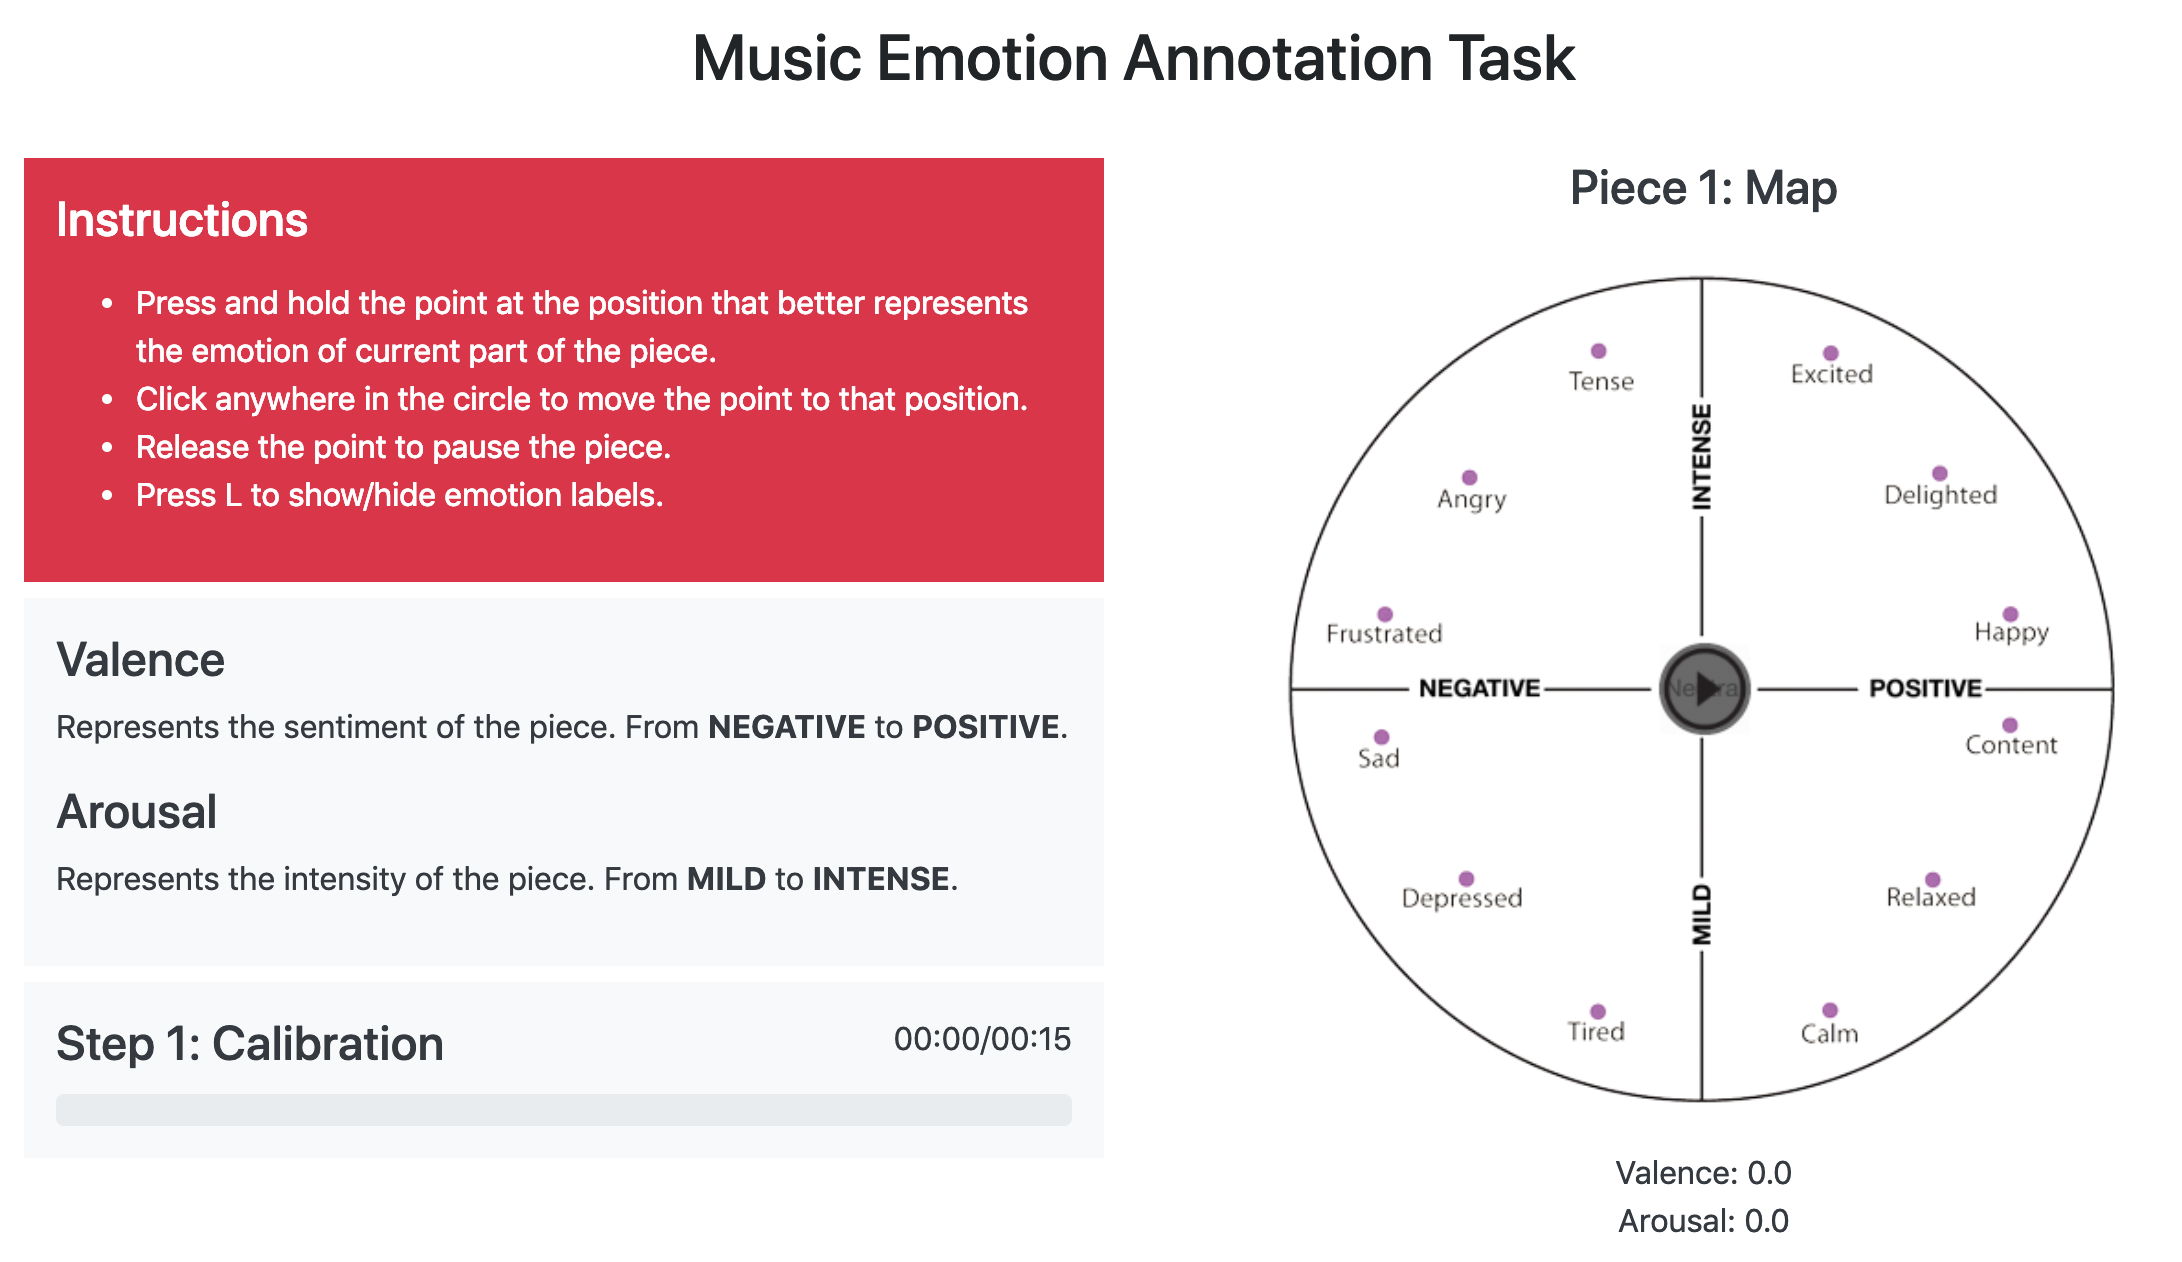
\includegraphics[width=\columnwidth]{imgs/ismir19/annotation_tool.png}
 \caption{Screenshot of the annotation tool.}
 \label{fig:annotation_main}
\end{figure}

\subsection{Data Analysis}
\label{sec:data_analysys}

The annotation task was performed by 1425 annotators, where 55\% are female and 42\% are male. The other 3\% classified themselves as transgender female, transgender male, genderqueer, or choose not to disclose their gender. All annotators are from the United States and have an average age of approximately 31 years. Musicianship experience was assessed using a 5-point Likert scale where 1 means ``I've never studied music theory or practice'' and 5 means ``I have an undergraduate degree in music''. The average musicianship experience is 2.28. They spent on average 12 minutes and 6 seconds to annotate the two pieces.

The data collection process provides a time series of valence-arousal values for each piece. However, only the valence dimension is needed to create a music sentiment dataset. Thus, each piece has 30 time series of valence values. The annotation of each piece was preprocessed, summarized into one time series, and split into ``phrases'' of the same sentiment. The preprocessing is intended to remove noise caused by subjects performing the task randomly to get the reward as fast as possible. The data was preprocessed by smoothing each annotation with a moving average and clustering all 30 time series into 3 clusters (positive, negative, and noise) according to the dynamic time-warping distance metric.

The cluster with the highest variance is considered noise, and so it is discarded. The cluster with more time series among the two remaining ones is then selected and summarized by the mean of its time series. The mean is split at all the points where the valence changes from positive to negative or vice-versa. This process creates several segments with the same sentiment, where segments with negative valence are considered negative phrases and segments with positive valence are positive phrases. Figure \ref{fig:clustering} shows an example of this three-step process performed on a piece. All the phrases that had no notes (i.e. silence phrases) were removed. This process created a total of 966 phrases: 599 positive and 367 negative.

\begin{figure}
 \centering
 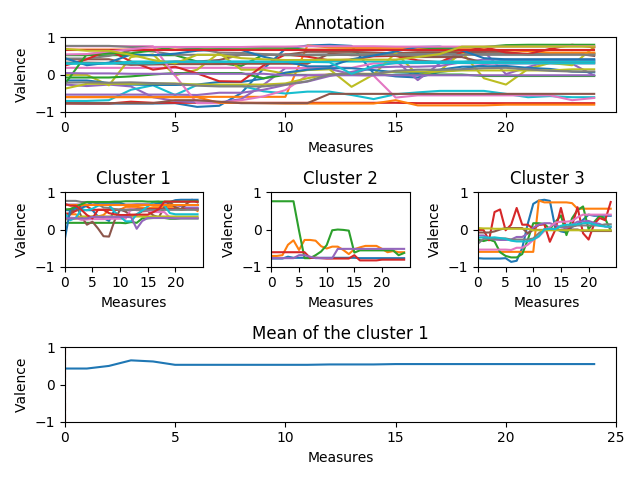
\includegraphics[width=\columnwidth]{imgs/ismir19/clustering.png}
 \caption{Data analysis process used to define the final label of the phrases of a piece. }
 \label{fig:clustering}
\end{figure}

% Table \ref{tab:dataset} shows a snippet of the dataset.
%
% \begin{table}[!h]
%  \begin{center}
%  \begin{tabular}{ccc}
%   \hline
%   \textbf{Label} & \textbf{Piece ID} & \textbf{MIDI Phrase} \\
%   \hline
%      0 & 14 & piece14\_phrase6.mid \\
%      0 & 14 & piece14\_phrase7.mid \\
%      1 & 15 & piece15\_phrase0.mid \\
%   \hline
%  \end{tabular}
% \end{center}
%  \caption{Snippet of the VGMIDI labeled phrases.}
%  \label{tab:dataset}
% \end{table}

\section{Models and Data Representation}
\label{sec:model}

% Deep Learning has recently achieved incredible results in music composition,
% but one still can't guide the proposed models to generate compositions
% with a given goal. This paper is motivated by the application of soundtrack
% generation and so it focus on the controlling emotions of the generated pieces.
% We propose a Deep Learning method for affective algorithmic composition that can be controlled to generate music with a given sentiment. This method is based on the work of Radford et al. \cite{radford_2017} which generates product reviews (in textual form) with sentiment.

Radford et al. \cite{radford_2017} used a single-layer multiplicative LSTM (mLSTM) network \cite{krause2017} with 4096 neurons to learn a character-based language model from a sequence of UTF-8 encoded characters. The trained mLSTM was fine-tuned with an extra linear layer to classify sentiment in text. During fine-tuning, the pre-trained weights of the mLSTM were kept frozen, and only the weights of the extra classification layer were trained. Moreover, L1 regularization was used during tine-tuning to enforce a sparse set of weights in the classification layer. This work uses the same models and training procedures to compose music with a target sentiment. Instead of characters, this work represents music pieces as sequences of tokens from a vocabulary representing events retrieved from MIDI files. Sentiment is perceived in music due to several features such as melody, harmony, tempo, and timbre\cite{kim2010music}. This data representation attempts to encode a large part of these features\footnote{Constrained by the features one can extract from MIDI data.} using a small set of words:

% The hidden state of the model
% serves as an online summary of the sequence which encodes all information
% the model has learned to preserve that is relevant to predicting the future
% bytes of the sequence.

% \begin{center}
% \begin{tikzpicture}
%     \draw[thick,->] (0,2) node[anchor=south] {input} -- (1,2);

%     \draw (1,1) -- (1.5,1) -- (1.5,3) -- (1,3)  -- (1,1);

%     \draw[thick,->] (1.5,2) node [anchor=south, rotate=90] {Embed.} -- (2.5,2);

%     \draw (2.5,0) -- (3,0) -- (3,4) -- (2.5,4) -- (2.5,0);

%     \draw[thick,->] (3,2) node [anchor=south, rotate=90] {mLSTM} -- (4,2);

%     \draw (4,1) -- (4.5,1) -- (4.5,3) -- (4,3) -- (4,1);

%     \draw[thick,->] (4.5,2) node [anchor=south, rotate=90] {Softmax} -- (5.5,2) node[anchor=south] {output};
% \end{tikzpicture}
% \captionof{figure}{Architecture of the mLSTM used to process text.}
% \label{fig:mlstm}
% \end{center}

% This mLSTM was trained on the Amazon product review dataset, which contains over 82 million product reviews from May 1996 to July 2014 amounting to over 38 billion training bytes \cite{He2016}. Radford et al. \cite{radford_2017} used the trained mLSTM to encode sentences from four different Sentiment Analysis datasets. The encoding is performed by initializing the the states to zeros and processing the sequence character-by character. The final hidden states of the mLSTM are used as a feature representation. With the encoded datasets, Radford et al. \cite{radford_2017} trained a simple logistic regression classifier with L1 regularization and outperformed the state-of-the-art methods at the time using 30-100x fewer labeled examples.
% By inspecting the relative contributions of features on various datasets,
% Radford et al. \cite{radford_2017} discovered a single unit within the
% mLSTM that directly corresponded to sentiment. Because the mLSTM was
% trained as a generative model, one can simply set the value of the
% sentiment unit to be positive or negative and the model generates
% corresponding positive or negative reviews.

\begin{itemize}
    \item ``n\_[pitch]'': play note with given pitch number: any integer from 0 to 127.
    \item ``d\_[duration]\_[dots]'': change the duration of the following notes to a given
    duration type with a given amount of dots. Types are breve, whole, half, quarter,
    eighth, 16th and 32nd. Dots can be any integer from 0 to 3.
    \item ``v\_[velocity]'': change the velocity of the following  notes to a given velocity (loudness) number. Velocity is discretized in
    bins of size 4, so it can be any integer in the set $V = {4, 8, 12, \dots, 128}$.
    \item ``t\_[tempo]'': change the tempo of the piece to a given tempo in bpm. Tempo is also discretized in bins of size 4, so it can be any integer in the set $T = {24, 28, 32, \dots, 160}$.
    \item ``.'': end of time step. Each time step is one sixteenth note long.
    \item ``\textbackslash n'': end of piece.
\end{itemize}

For example, Figure \ref{fig:enc_ex} shows the encoding of the first two time steps of the first measure of the Legend of Zelda - Ocarina of Time's Prelude of Light. The first time step sets the tempo to 120bpm, the velocity of the following notes to 76, and plays the D Major Triad for the duration of a whole note. The second time step sets the velocity to 84 and plays a dotted quarter A5 note. The total size of this vocabulary is 225, and it represents both the composition and performance elements of a piece (timing and dynamics).

\begin{figure}
 \centering
 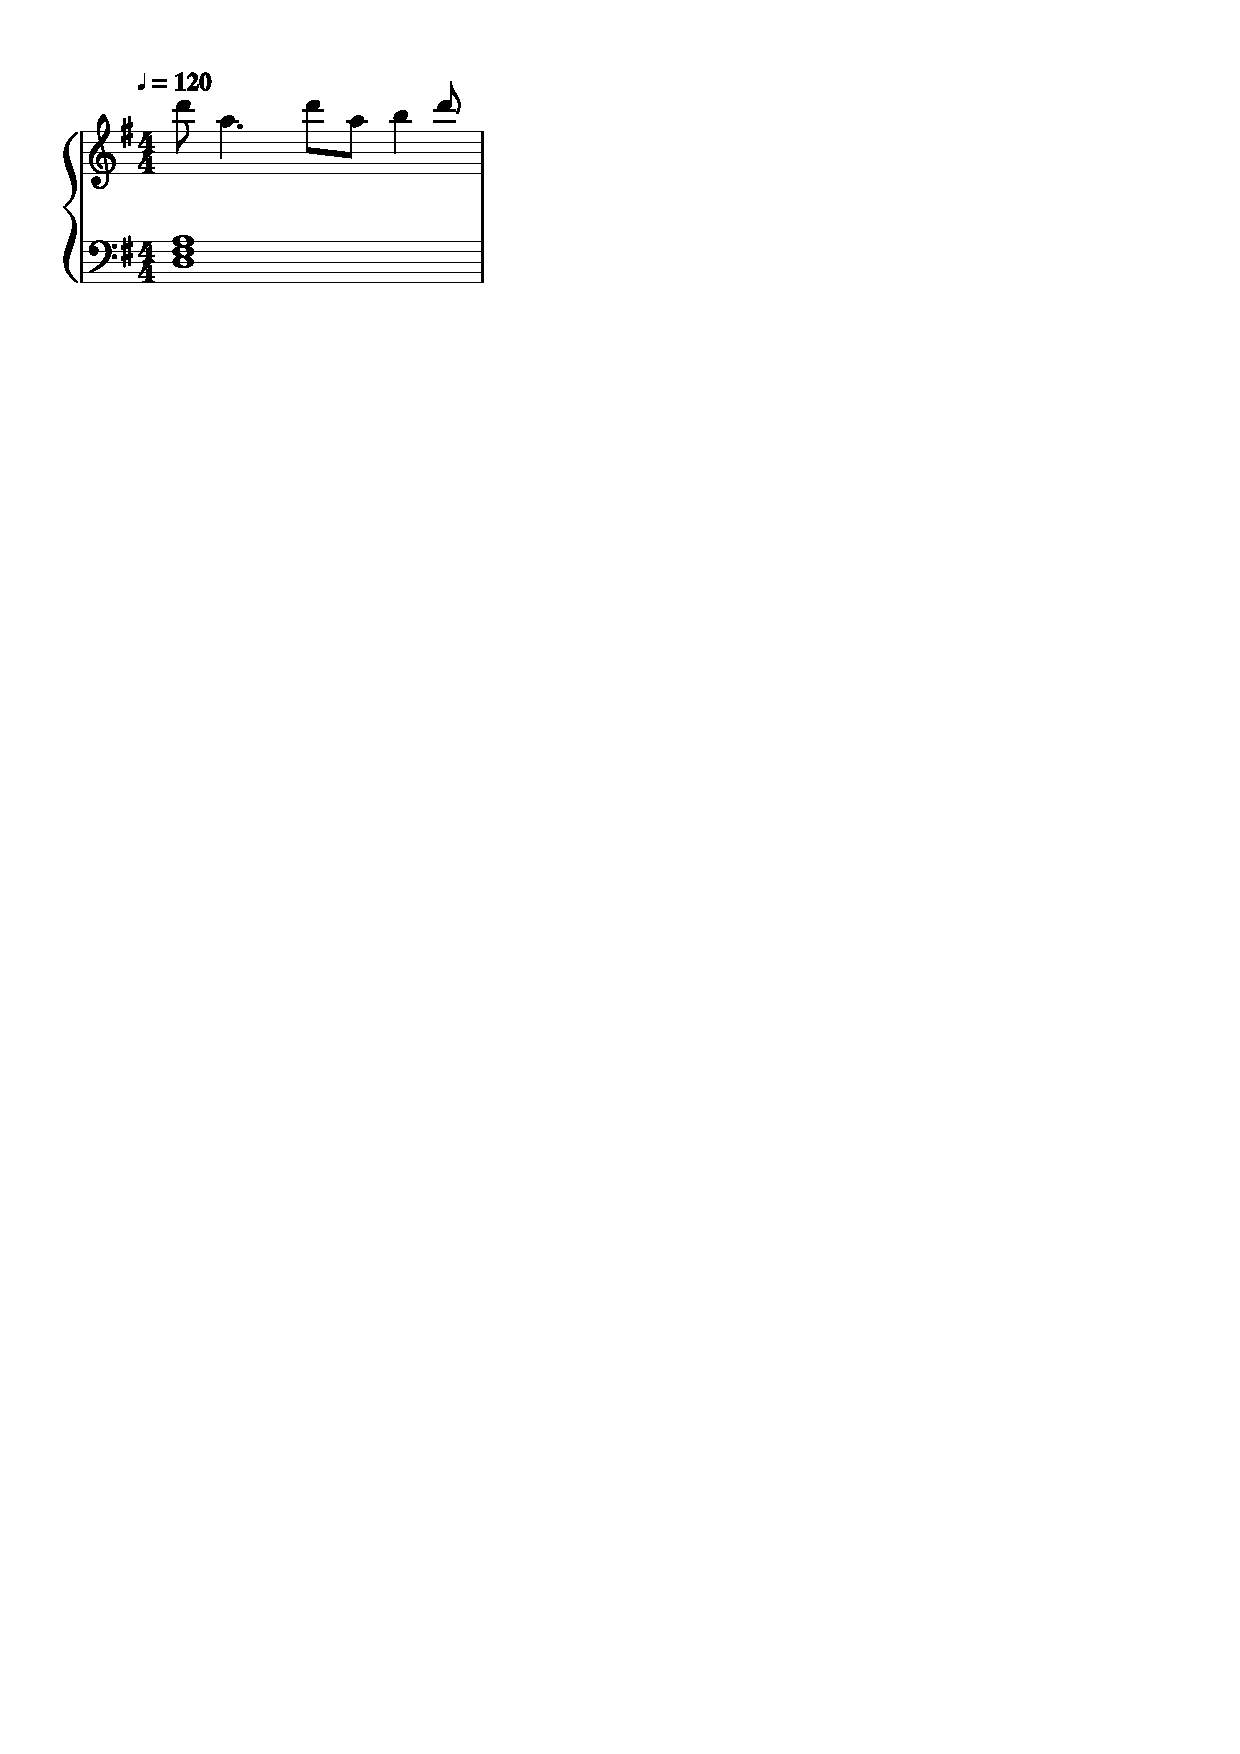
\includegraphics[width=.95\columnwidth]{imgs/ismir19/encoding.pdf}
\begin{spverbatim}
        t_120 v_76 d_whole_0 n_50 n_54 n_57 v_92 d_eighth n_86 . . v_84
        d_quarter_1 n_81 . .
\end{spverbatim}

 \caption{A short example piece encoded using the proposed representation. The encoding represents the first two time steps of the shown measure.}
 \label{fig:enc_ex}
\end{figure}

\section{Sentiment Analysis Evaluation}

The fine-tuning approach (LM + linear sentiment classification layer) proposed in this work is initially evaluated in the sentiment classification task. First, a mLSTM LM is pre-trained with the unlabelled pieces of the VGMIDI dataset. Then, the pre-trained LM layers are frozen, and an additional linear layer is stacked on top of it. The resulting model is trained as a sentiment classifier with the labeled pieces of the VGMIDI dataset. This fine-tuned LM model was compared against a baseline mLSTM network trained directly on the supervised sentiment classification task. The baseline method uses only labeled MIDI phrases to train a classification mLSTM to predict the sentiment for the phrase.

The unlabelled pieces used to train the LM were augmented in order to create additional training examples, following the methodology of Oore et al. \cite{oore2017learning}. The augmentation consists of time stretching (making each piece up to 5\% faster or slower) and transposition (raising or lowering the pitch of each piece by up to a major third). All these pieces and transformations are encoded according to the proposed word-based representation (see Section \ref{sec:representation}). Finally, the encoded pieces were shuffled, and 90\% of them were used for training and 10\% for testing. The training set was divided into three shards of similar size (approximately 18,500 pieces each -- 325MB), and the testing set was combined into one shard (approximately 5800 pieces -- 95MB).

Six different sizes (number of neurons in the mLSTM layer) were compared for the LM: 128, 256, 512, 1024, 2048, and 4096. For each size, the LM was trained for 4 epochs using the 3 training shards. Weights were updated with the Adam optimizer after processing sequences of 256 words on mini-batches of size 32. The mLSTM hidden and cell states were initialized to zero at the beginning of each shard. They were also persisted across updates to simulate full-backpropagation and allow for the forward propagation of information outside of a given sequence \cite{radford_2017}. Each sequence is processed by an embedding layer (which is trained together with the mLSTM layer) with 64 neurons before passing through the mLSTM layer. The learning rate was set to $5*10^6$ at the beginning and decayed linearly (after each epoch) to zero over the course of training.

Each variation of the LM was evaluated with a forward pass on the test shard using mini-batches of size 32. Table \ref{tab:gen_anal} shows the average\footnote{Each mini-batch reports one loss.} cross entropy loss for each variation of the mLSTM LM. The average cross entropy loss decreases as the size of the mLSTM increases, reaching the best result (loss 1.11) when size is equal to 4096. Thus, the variation with 4096 neurons was used to proceed with the sentiment classification experiments.

\begin{table}[!h]
 \begin{center}
 \begin{tabular}{cc}
  \hline
  \textbf{mLSTM Neurons} & \textbf{Average Cross Entropy Loss}\\ \hline
  128 & 1.80   \\
  256  & 1.61  \\
  512  & 1.41  \\
  1024 & 1.25  \\
  2048 & 1.15  \\
  4096 & 1.11  \\ \hline
 \end{tabular}
\end{center}
\caption{Average cross entropy loss of the generative mLSTM with different amount of neurons.}
 \label{tab:gen_anal}
\end{table}

After training the LM, an extra linear sentiment classification layer is stacked on top of the base LM and trained with the 966 labeled phrases of the VGMIDI dataset. Here, stacking means passing the final cell states of the mLSTM as input to the linear classification layer. During this fine-tuning step, the base layers of the LM are frozen, which means only the weights of the stacked classification layer are updated. Moreover, these extra layer is trained with L1 regularization to shrink the least important of the 4096 feature weights to zero. This ends up highlighting the generative mLSTM neurons that contain most of the sentiment signal.

The fine-tuning approach (LM + linear sentiment classification layer) was compared against the baseline supervised mLSTM. This is an mLSTM with exactly the same architecture and size as the fine-tuned version but trained in a fully supervised way. This supervised mLSTM was trained with the same word-based representation of the phrases, but they were padded with silence (the symbol ``.'') in order to equalize their length. Training parameters were set to be the same used to train the base LM. Both methods were evaluated using a 10-fold cross-validation approach, where the test folds have no phrases that appear in the training folds. Table \ref{tab:sent_anal} shows the sentiment classification accuracy of both approaches.

\begin{table}[!h]
 \begin{center}
 \begin{tabular}{lc}
  \hline
  \textbf{Method} & \textbf{Test Accuracy} \\ \hline
  Fine-tuned mLSTM-4096 & 89.83 $\pm$ 3.14\\
  Baseline  mLSTM-4096 & 60.35 $\pm$ 3.52 \\
  \hline
 \end{tabular}
\end{center}
\caption{Average (10-fold cross validation) sentiment classification accuracy of both generative (with logistic regression) and supervised mLSTMs.}
 \label{tab:sent_anal}
\end{table}

The fine-tuned mLSTM achieved an accuracy of 89.83\%, outperforming the supervised mLSTM by 29.48\%. The supervised mLSTM accuracy of 60.35\% suggests that the amount of labeled data (966 phrases) was not enough to learn a good mapping between phrases and sentiment. The accuracy of the fine-tuned mLSTM shows that it is capable of learning, in an unsupervised way, a good representation of sentiment in symbolic music. This is an important result for two reasons. First, since the higher accuracy of fine-tuned mLSTM is derived from unlabeled data, it will be easier to improve this over time using additional (less expensive) unlabeled data instead of the supervised mLSTM approach, which requires additional (expensive) labeled data. Second, because the mLSTM LM was trained to predict the next word in a sequence, it can be used as a music generator. Since it is combined with a sentiment predictor, it opens up the possibility of generating music consistent with a desired sentiment. This idea is explored in the following section.

\section{Generative Evaluation}

To control the sentiment of the music generated by the fine-tuned mLSTM, one has to find the subset of neurons that contain the sentiment signal by exploring the weights of the linear sentiment classification layer. As shown in Figure \ref{fig:final_weights}, the linear classification layer trained with L1 regularization uses 161 neurons out of 4096. Unlike the results of Radford et al. \cite{radford_2017}, the fine-tuning step did not store the sentimental in a single neuron. Instead, the sentiment signal was stored across many neurons in a more balanced way. Therefore, one cannot simply change the values of one neuron to control the sentiment of the output music.

\begin{figure}[!h]
 \centering
 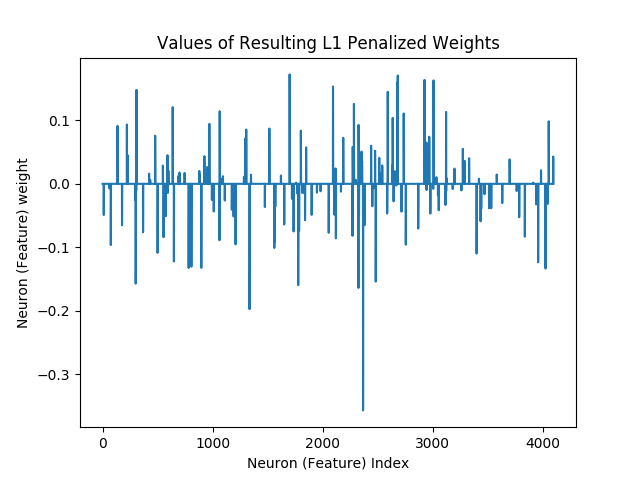
\includegraphics[width=\columnwidth]{imgs/ismir19/weights.png}
 \caption{Weights of 161 L1 neurons. Note multiple prominent positive and negative neurons.}
 \label{fig:final_weights}
\end{figure}

A Genetic Algorithm (GA) was used to optimize the 161 L1 neurons' weights to lead the fine-tuned mLSTM to generate only positive or negative pieces. Each individual in the population of this GA has $161$ real-valued genes representing a small noise to be added to the weights of the $161$ L1 neurons. The fitness of an individual is computed by (i) adding the genes of the individual to the weights (vector addition) of the $161$ L1 neurons of the generative mLSTM, (ii) generating $P$ pieces with this mLSTM, (iii) using the logistic regression model to predict these $P$ generated pieces and (iv) calculating the mean squared error of the $P$ predictions given a target sentiment $s \in S = \{0, 1\}$.

The GA starts with a random population of size 100 where each gene of each individual is a uniformly sampled random number $-2 \leq r \leq 2$. For each generation, the GA (i) evaluates the current population, (ii) selects 100 parents via a roulette wheel with elitism, (iii) recombines the parents (crossover) taking the average of their genes, and (iv) mutates each new recombined individual (new offspring) by randomly setting each gene to a uniformly sampled random number $-2 \leq r \leq 2$.

This GA was executed twice: once to optimize the fine-tuned mLSTM for generating positive pieces and once for negative pieces. Each execution optimized the individuals during 100 epochs with a crossover rate of 95\% and mutation rate of 10\%. To calculate each individual's fitness, $P$=30 pieces were generated with 256 words each, starting with the symbol ``.'' (end of time step). The optimization for positive and negative generation resulted in best individuals with fitness $0.16$ and $0.33$, respectively. This means that if one adds the genes of the best individual of the final population to the weights of the generative mLSTM, one generates positive pieces with 84\% accuracy and negative pieces with 67\% accuracy.

After these two optimization processes, the genes of the best final individual of the positive optimization were added to the weights of the 161 L1 neurons of the trained LM. A set of 30 pieces was then generated with 1000 words starting with the symbol ``.'' (end of time step) and 3 of them were randomly selected. The same process was repeated using the genes of the best final individual of the negative execution. Annotators were asked to label these 6 generated pieces via Amazon MTurk, using the same methodology described in Section \ref{sec:data_collection}. Figure \ref{fig:generated_eval} shows the average valence per measure of each of the generated pieces.

\begin{figure}[!h]
 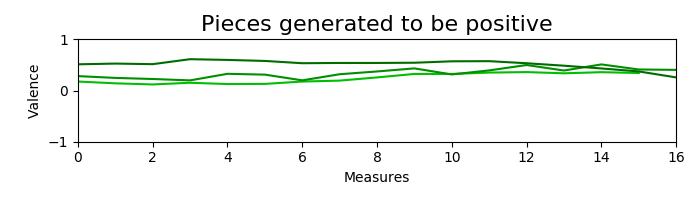
\includegraphics[width=\columnwidth]{imgs/ismir19/means_pos.png}
 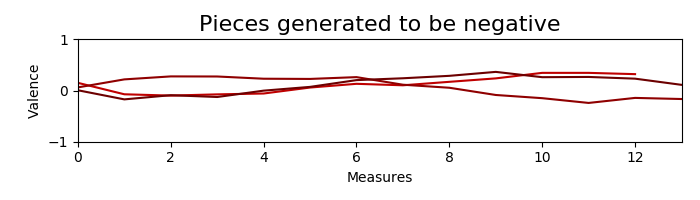
\includegraphics[width=\columnwidth]{imgs/ismir19/means_neg.png}
 \caption{Average valence of the 6 generated pieces, as determined by human annotators.
 %Note that the averages are calculated after clustering the annotations and selecting the cluster
 with least variance.}
 \label{fig:generated_eval}
\end{figure}

These results showed that human annotators agreed that the three positive generated pieces are indeed positive. The generated negative pieces are more ambiguous, having both negative and positive measures. However, as a whole, the negative pieces have lower valence than the positive ones. This suggests that the best negative individual (with fitness $0.33$) encountered by the GA was not good enough to control the mLSTM to generate complete negative pieces. Moreover, the challenge to optimize the L1 neurons suggests that there are more positive pieces than negative ones in the 3 shards used to train the generative mLSTM.

\section{Conclusions}

This chapter presented a mLSTM LM that can be controlled to generate symbolic music with a given sentiment. The mLSTM is controlled with a genetic algorithm that optimizes the weights of specific neurons that are responsible for the sentiment signal. Such neurons are found by fine-tuning the mLSTM with an extra linear layer to classify the sentiment of symbolic music. This fine-tuning approach was evaluated both as a generator and as a sentiment classifier. Results showed that the fine-tuned mLSTM obtained good classification accuracy, outperforming an equivalent mLSTM trained in a fully supervised way. Moreover, a user study showed that humans agree that the fine-tuned LM can generate positive and negative music, with the caveat that the negative pieces are more ambiguous than the positive ones.

% The next chapter presents another search-based approach to control emotion (not only sentiment) in music generated by a LM. This new method was applied to compose background music in real-time for tabletop role-playing games\cite{padovani2017bardo}.
